\usetikzlibrary{arrows.meta}
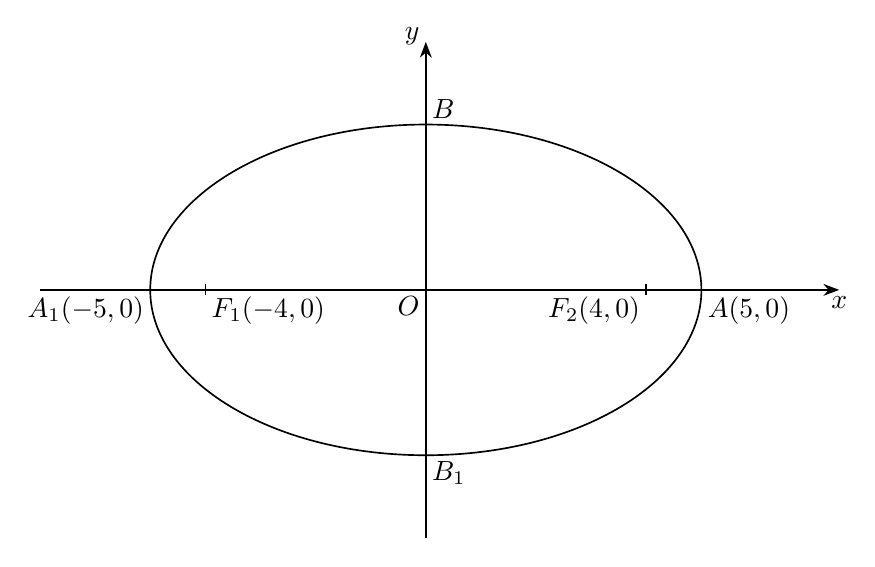
\begin{tikzpicture}[x=0.7cm,y=0.7cm,line width=.6pt,font=\normalsize,>=Stealth]
\draw[->] (-7,0)--(7.5,0);
\draw[->] (0,-4.5)--(0,4.5);
\draw (0,0) ellipse[x radius=3.5cm,y radius=2.1cm];
\draw[line width=.6pt] (-4,0.1)--(-4,-0.1);
\draw[line width=.6pt] (4,0.1)--(4,-0.1);
\node[anchor=north east,inner sep=0pt,xshift=-2pt,yshift=-2pt] at (-5,0) {$A_{1}(-5,0)$};
\node[anchor=north west,inner sep=0pt,xshift=2pt,yshift=-2pt] at (-4,0) {$F_{1}(-4,0)$};
\node[anchor=north east,inner sep=0pt,xshift=-2pt,yshift=-2pt] at (0,0) {$O$};
\node[anchor=north east,inner sep=0pt,xshift=-2pt,yshift=-2pt] at (4,0) {$F_{2}(4,0)$};
\node[anchor=north west,inner sep=0pt,xshift=2pt,yshift=-2pt] at (5,0) {$A(5,0)$};
\node[anchor=south west,inner sep=0pt,xshift=2pt,yshift=2pt] at (0,3) {$B$};
\node[anchor=north west,inner sep=0pt,xshift=2pt,yshift=-2pt] at (0,-3) {$B_{1}$};
\node[anchor=north,inner sep=0pt,yshift=-2pt] at (7.5,0) {$x$};
\node[anchor=east,inner sep=0pt,xshift=-2pt,yshift=2pt] at (0,4.5) {$y$};
\end{tikzpicture}
